\section{Increasing Number of Agent Iterations}
\label{appendix_sec:increasing_n_iterations}
\begin{figure*}[thbp]
\centering
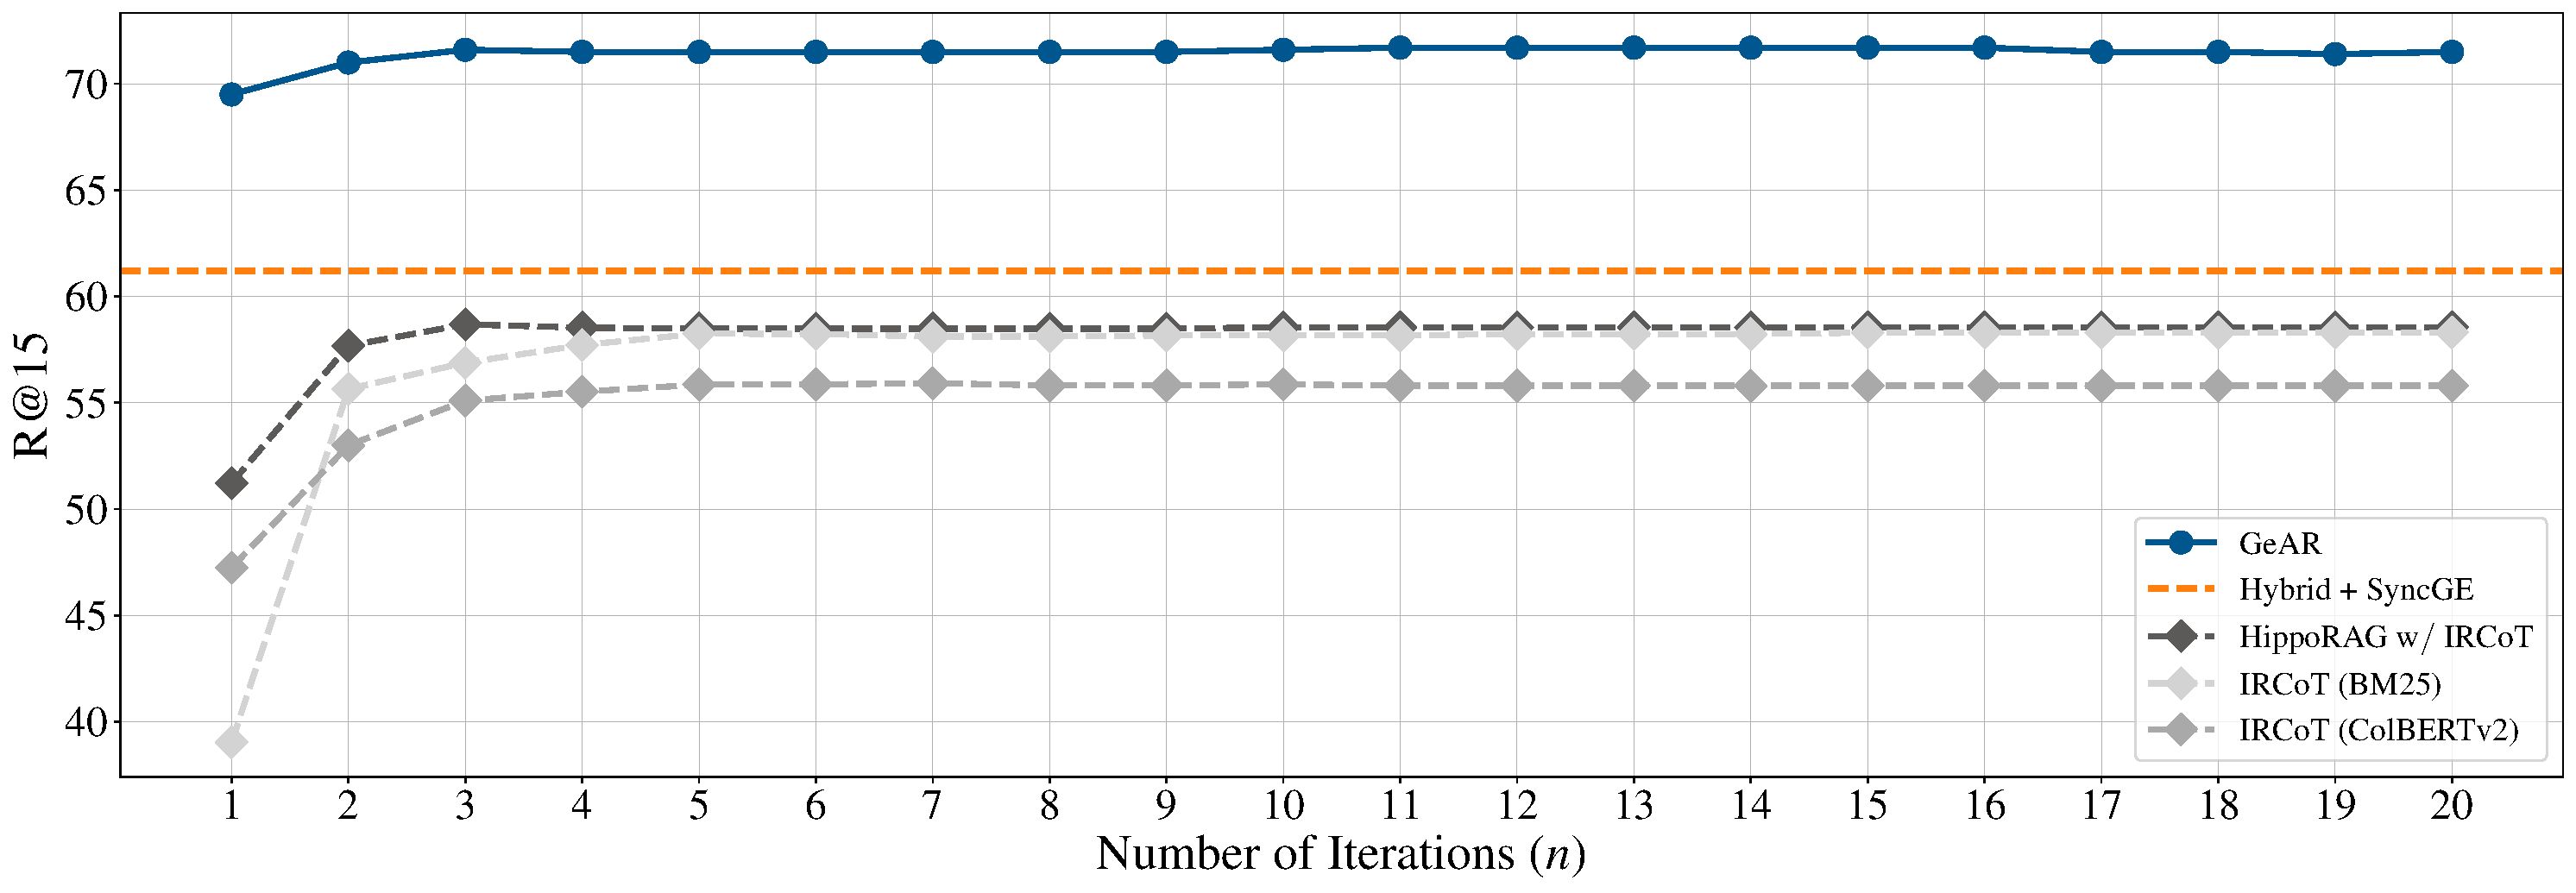
\includegraphics[width=\textwidth]{figures/experiments/recall_evolution_across_agent_iterations_20_iters.pdf}
\caption{Evolution of R@15 over 20 iterations on MuSiQue. Recall is computed at each iteration using the cumulative set of retrieved documents, with prior recall values carried forward for questions that terminated in earlier iterations. The horizontal line indicates the single-step performance of Hybrid + SyncGE.}
\label{fig:recall_across_iterations_20_iters}
\end{figure*}

Figure \ref{fig:recall_across_iterations_20_iters} expands upon the analysis shown in Figure \ref{fig:recall_across_iterations} by evaluating retrieval performance over 20 iterations, rather than the initial 4 iterations. The results demonstrate a consistent pattern across all methods: retrieval performance stabilises after approximately 4 iterations, with no substantial improvements or degradation in subsequent iterations. While some minor fluctuations occur beyond this point, they are negligible.

This performance plateau can be attributed to two key factors. First, the query re-writing mechanisms in all investigated approaches struggle to generate effective subsequent queries. Second, our analysis has identified several cases of unanswerable queries within MuSiQue's answerable subset. A representative example is provided in Table~\ref{tab:musique_problematic_example}.


\begin{table*}
\centering
\footnotesize
\begin{tabular}{L{3cm}L{12cm}}

\toprule
\textbf{Question} & Who did the \textcolor{red}{producer} of \textcolor{purple}{Big Jim McLain} play in \textcolor{purple}{True Grit}? \\
\midrule
\multirow{3.5}{*}{\textbf{Gold Passages}} & {1. \textcolor{purple}{Big Jim McLain}: \textcolor{purple}{Big Jim McLain} is a 1952 political thriller film starring John Wayne and James Arness as HUAC investigators.}\\\cmidrule{2-2}
& {2. \textcolor{purple}{True Grit} is a 1969 American western film. It is the first film adaptation of Charles Portis' 1968 novel of the same name. The screenplay was written by Marguerite Roberts. The film was directed by Henry Hathaway and starred Kim Darby as Mattie Ross and John Wayne as U.S. Marshal Rooster Cogburn. Wayne won his only Academy Award for his performance in this film and reprised his role for the 1975 sequel Rooster Cogburn.}\\
\midrule
\textbf{Comment} & \textcolor{red}{No information about who was the producer of} \textcolor{purple}{Big Jim McLain} \textcolor{red}{is provided in the gold passages}\\
\bottomrule
\end{tabular}
\caption{\label{tab:musique_problematic_example}Example of a query from MuSiQue that in not answerable solely based on the provided gold passages.}
\end{table*}
